\chapter{Теоретический базис} \label{chapt1}
В настоящей главе будут представлены элементы статистической оптики, а именно одна из основных теорем статистической оптики, теорема Ван Циттерта - Цернике. Используя вывод теоремы, в качестве примера оценивается пятно когерентности излучения для рентгеновской трубки -- полностью некогерентного источника излучения. Далее даётся формулировка обобщённой теоремы Ван Циттерта - Цернике в случае, когда на источнике излучения есть конечная область когерентности, или, другими словами, источник частично когерентен. В главе рассматриваются вопросы формирования синхротронного излучения от электронного сгустка с конечным эмиттансом. Описываются статистические свойства такого излучения и характерная спайковая структура излучения для одной статистической реализации поля.
\section{Поперечная функция когерентности и теорема Ван Циттерта - Цернике}
Поперечная функция когерентности в плоскости $z = const$ имеет вид:
\begin{align}
	\Gamma^{(1)}_{\perp} (\vec{r}_1, \vec{r}_2, \omega, z) = \big \langle {E}^*(\vec{r}_1, \omega, z) {E}(\vec{r}_2, \omega, z) \big \rangle,
	%	\sqrt{\big \langle |{E}(r_1, t)|^2\big \rangle \big \langle|{E}(r_2, t)|^2 \big \rangle}}, 
	\label{eq:g1} 
\end{align}
где -- $\big \langle ... \big \rangle$ означает усреднение по ансамблю реализаций спектральных амплитуд монохроматического поля $\bar{E}(\vec{r}, \omega, z)$ от некоторого некогерентного стационарного источника излучения. Связь функции поперечной когерентности $\Gamma^{(1)}_{\perp} (\vec{r}_1, \vec{r}_2, \omega, z)$ с распределением интенсивности источника излучения $I(\xi, \eta)$ даётся двумерным преобразованием Фурье, что является следствием теоремы Ван Циттерта - Цернике ~\cite{van_cittert_wahrscheinliche_1934},~\cite{zernike_concept_1938}:
\begin{align}
	\Gamma^{(1)}_{\perp} (\vec{r}_1, \vec{r}_2, \omega, z) = \cfrac{\kappa e^{-i\psi}}{({\lambda}z)^2} \iint \limits_{-\infty}^{+\infty} I(\xi, \eta) \exp{\big [(i \cfrac{2 \pi}{{\lambda}z}) (\Delta x \xi + \Delta y \eta)\big]}d\xi d\eta, 
	\label{eq:van_cittert_zernike_theorem} 
\end{align}
где $\kappa = {\lambda}^2 / \pi$, ${\lambda}$ -- длина волны монохроматического источника излучения\footnote{В оригинальной работе теорема формулируется для квазимонохроматического источника. Для простоты мы опускаем эту общую формулировку и сужаем теорему для монохроматических источников.}, $z$ -- расстояние до плоскости наблюдения от источника излучения, $\psi = \cfrac{\pi}{{\lambda} z}\big[((x^2_2 + y^2_2) - (x^2_1 + y^2_1)) \big]$, а $\Delta x = x_2 - x_1$, $\Delta y = y_2 - y_1$, другие геометрические величины изображены на Рис.~\ref{fig:VCC_scheme_incoh}.
\begin{figure}[H] 
	\centering 	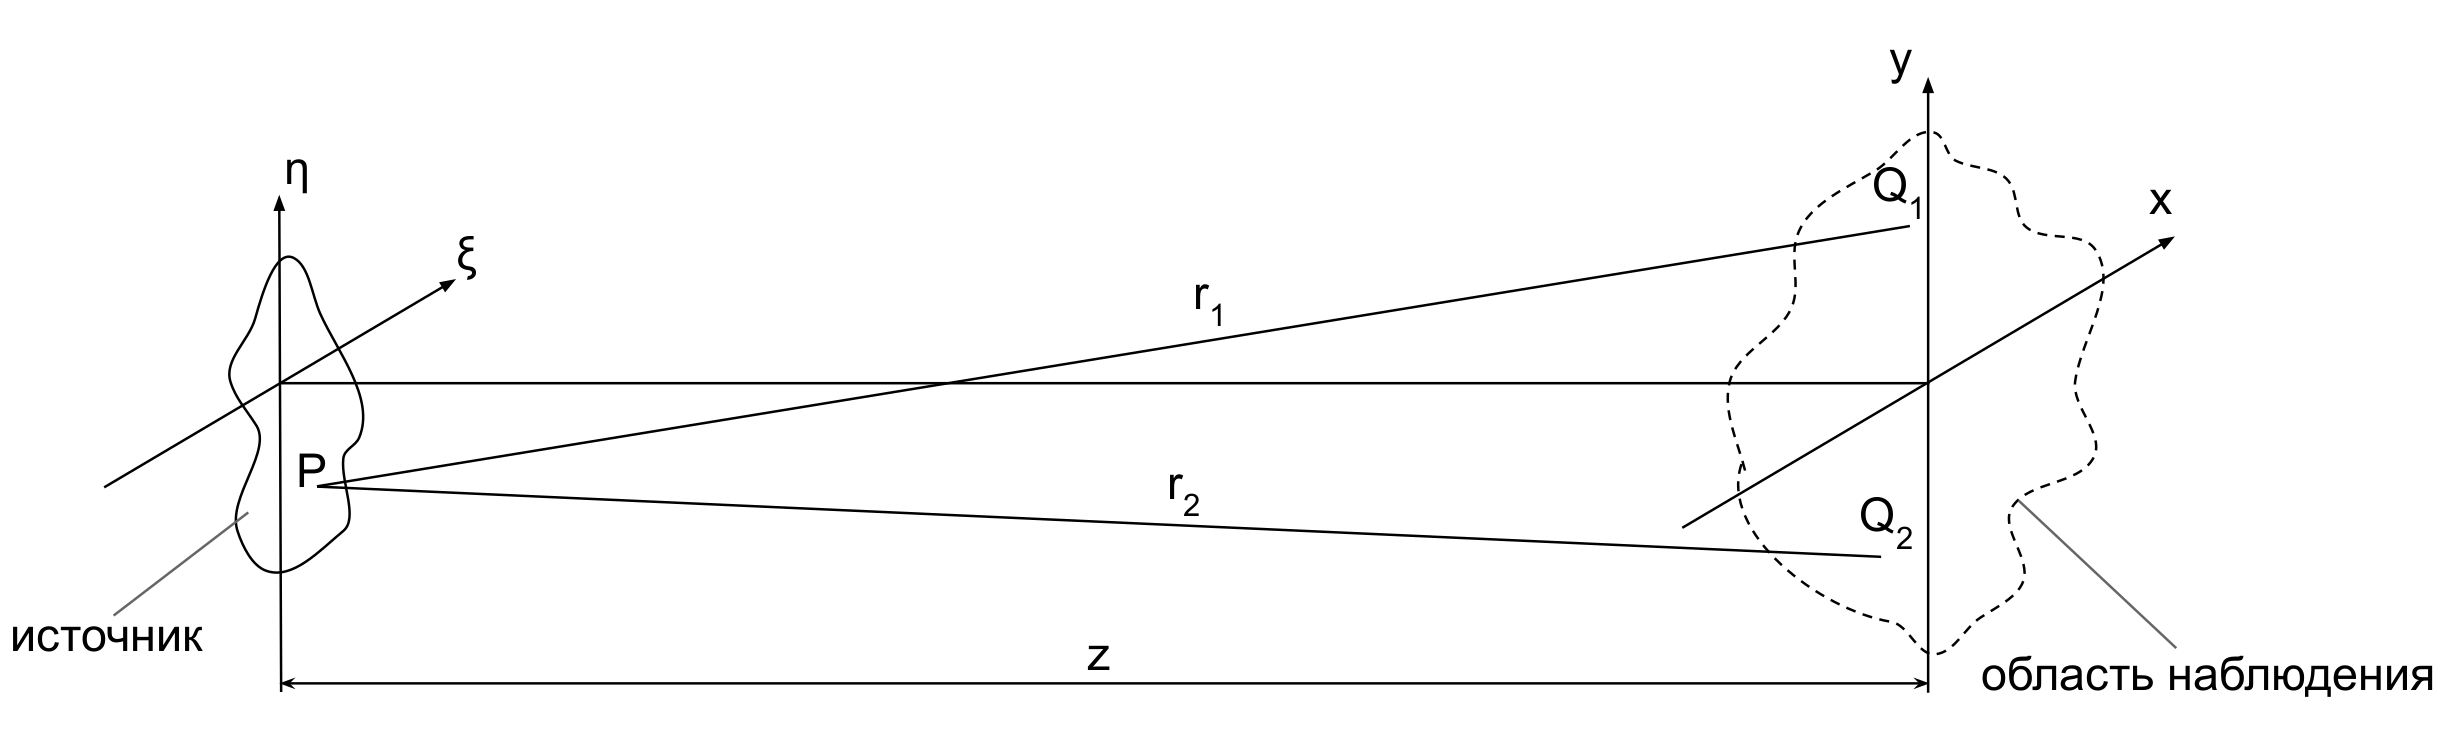
\includegraphics[width=0.99\linewidth]{VCC_incoh_scheme.png}
	\caption{К формулировке теоремы Ван Циттерта-Цернике}
	\label{fig:VCC_scheme_incoh}
\end{figure}
Таким образом, площадь пятна когерентности на расстоянии $z$ от источника будет определяться следующим выражением:
\begin{align}
	A_c = \cfrac{({\lambda} z)^2}{A_s}.
	\label{eq:VCC}
\end{align}

Теорема может быть видоизменена и обобщена для частично когерентных источников излучения, достаточно лишь заменить $\kappa$ на двойной интеграл \cite{goodman_statistical_2015}
\begin{align}
	\kappa(\bar{x}, \bar{y}) = \iint \limits_{-\infty}^{+\infty} \mu(\Delta \xi, \Delta \eta) \exp{\big [(i \cfrac{2 \pi}{{\lambda}z}) ( \bar{x} \Delta \xi + \bar{y} \Delta \eta)\big]}d\Delta \xi d\Delta \eta, 
\end{align}
где $\bar{x} = \cfrac{x_1 + x_2}{2}, \bar{y} = \cfrac{y_1 + y_2}{2}$,  $\Delta \xi = \xi_2 - \xi_1$, $\Delta \eta = \eta_2 - \eta_1$ и $\mu(\Delta \xi, \Delta \eta)$ -- комплексный коэффициент когерентности, являющийся областью когерентности на источнике. Физически это означает следующее: усреднённое распределение интенсивности излучения в дальней зоне будет обратно пропорциональна пятну когерентности излучения на источнике, а характерный размер когерентности в плоскости $z = const$ обратно пропорционален размеру источника излучения (Рис.~\ref{fig:VCC_scheme_partially}).
\begin{figure}[H] 
	\centering 	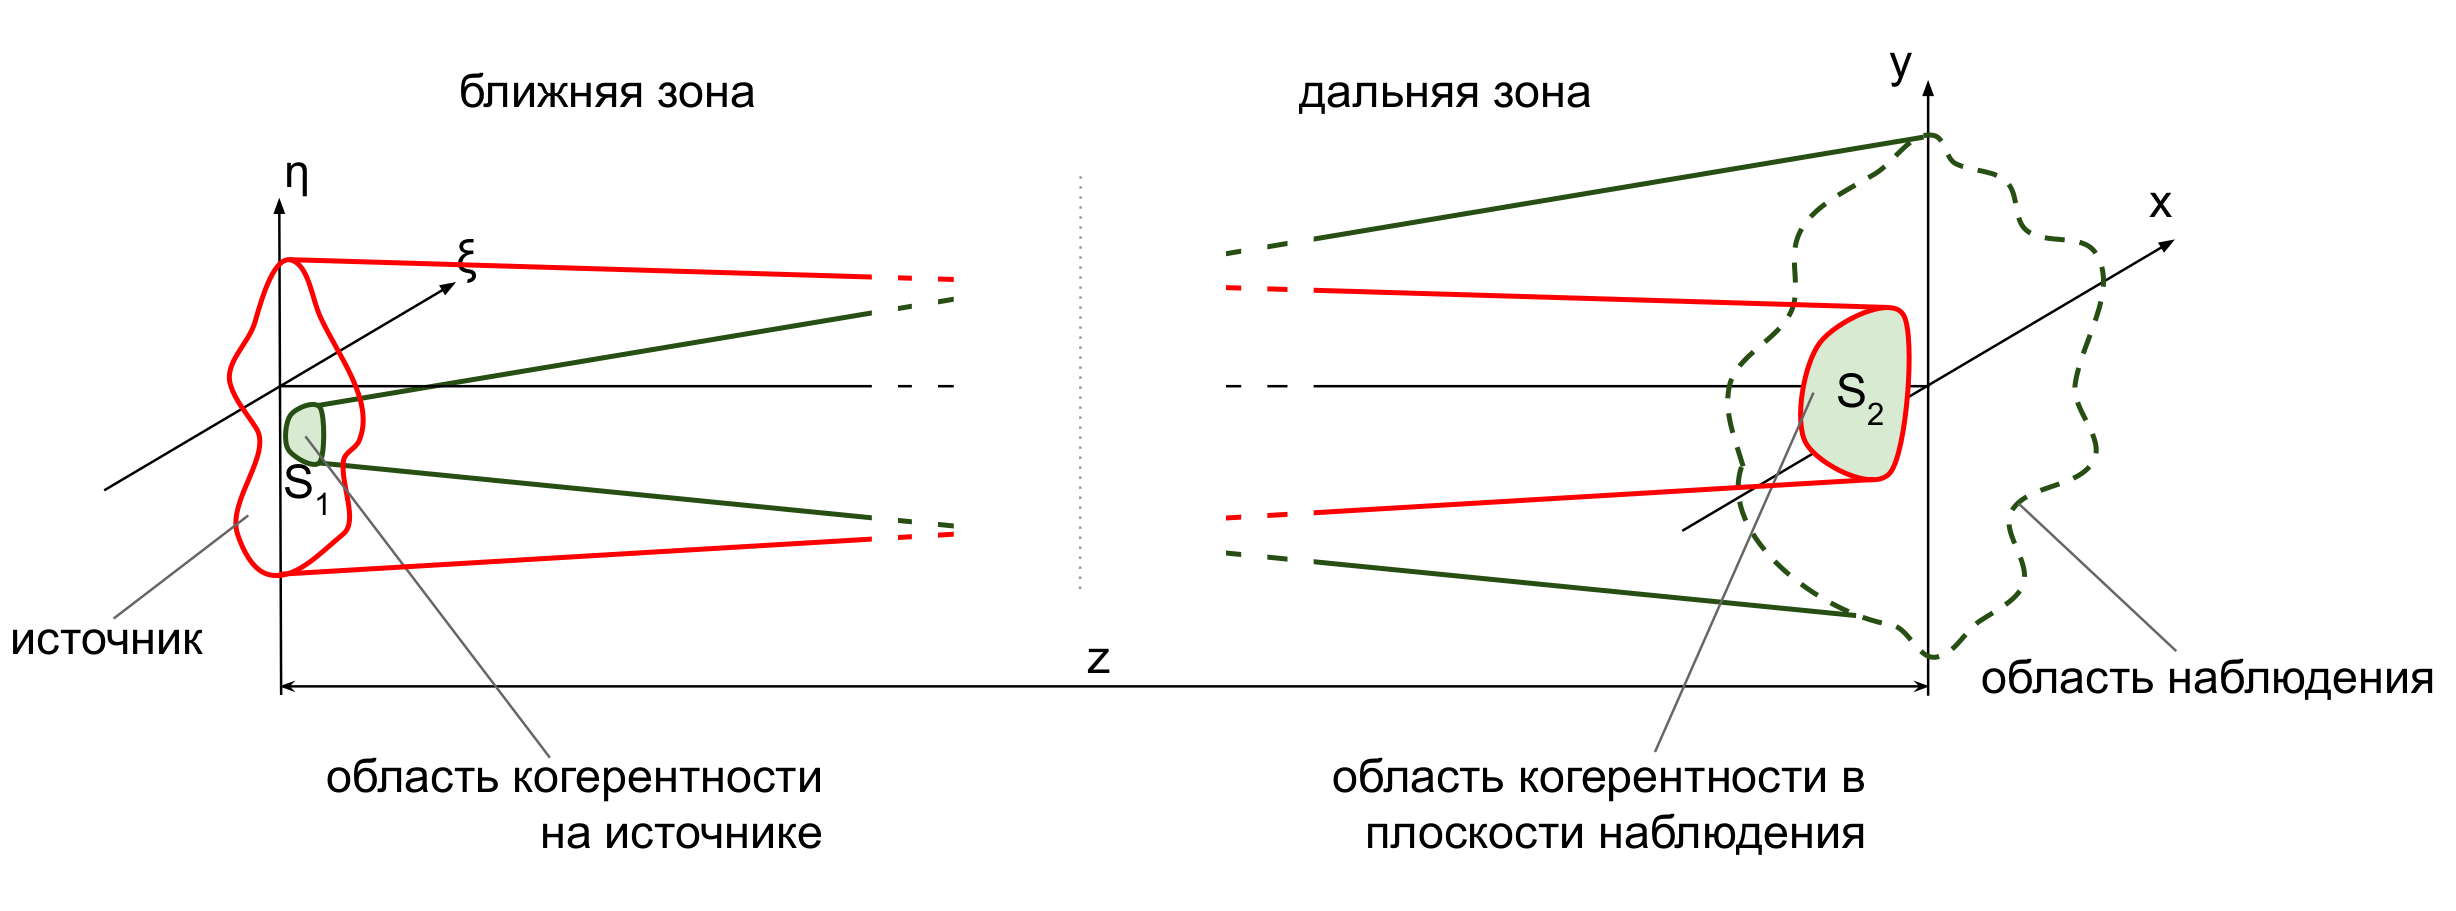
\includegraphics[width=0.99\linewidth]{VCC_partially_coh_scheme.png}
	\caption{К формулировке обобщённой теоремы \\ Ван Циттерта-Цернике}
	\label{fig:VCC_scheme_partially}
\end{figure}

В качестве примера распространения когерентности от полностью некогерентного источника можно оценить область когерентности излучения лабораторной рентгеновской трубки на некотором расстоянии $z$. Область когерентности от полностью некогерентного источника излучения квадратной формы получается напрямую из теоремы Ван Циттерта-Цернике. Подставляя в уравнение~\ref{eq:VCC} $z = 1$ м, $\lambda \approx 0.7$ $\textup{\AA}$ и площадь фокального пятна\footnote{Площадь фокального пятна спроецирована на направление выхода излучения из рентгеновской трубки.} $A_s = 1$ $\textup{мм}^2$, \cite{cullity_elements_1956}, получаем, что линейный размер длины когерентности при отражении от кристалла будет порядка\footnote{С учётом угла дифракции ($\sim 45^{\circ}$).} $0.1$ $\textup{мкм}$. Линейный размер пятна когерентности может быть увеличен до нескольких микрон при использовании трубки с вращающимся анодом, где характерный размер источника достигает $50$ $\textup{мкм}$ \cite{cullity_elements_1956}.  

Для синхротронных источников излучения область когерентности на источнике определяется натуральным размером излучения одного электрона при пролёте через вставное устройство. В случае ондуляторного источника, натуральный размер излучения определяется геометрическим размером перетяжки излучения в центре ондулятора -- $\sigma_r = \sqrt{\lambda L}/4 \pi$, где $L$ длина ондулятора. Дальнейшие рассуждения о статистических свойствах синхротронного представлены в следующем разделе, а точные выражения представлены в~\cite{geloni_transverse_2008}. 

\section{О статистических свойства синхротронного излучения}
Излучение от всего электронного сгустка может быть представлено, как сумма полей от каждого электрона, где $k$-ый электрон в сгустке имеет свою координату -- $\vec{\eta}_k$, угол -- $\vec{\l}_k$, отсчитываемые от проектной траектории, а также время прибытия $t_k$ относительно некоторого времени $t_0$. Ондуляторное излучение удобно рассматривать в $\omega$-пространстве, т.е. $\bar{E}(\vec{r}, \omega)$, которое связано с полем $E(\vec{r}, t)$ обратным преобразованием Фурье по времени. Вклад времени прибытия в $r\omega$-пространстве будет простым умножением поля на фазовый фактор $\exp{(i \omega t_k)}$. Указанные величины $\vec{\eta}_k$, $\vec{\l}_k$ и $t_k$ подчиняются некоторым распределениям плотности вероятности, для накопительных колец в модельных случаях это распределение Гаусса. В настоящей работе не рассматриваются эффекты, связанные с влиянием разброса электронов по энергии на когерентные свойства излучения, эти эффекты описаны в \cite{geloni_effects_2018}. 

Результирующее поле от $N_e$ электронов на расстоянии $z$ от источника можно записать следующим образом:
\begin{align}
	\bar{E}_{b} (z, \omega, \vec{r}_{\bot}) = \sum\limits_{k=1}^{N_e} \bar{E}_{\bot}(&z_0, \omega, \vec{\eta}_k, \vec{\l}_k, \vec{r}_{\bot}) \exp{(i \omega t_k)},
	\label{eq:E_bunch} 
\end{align}
для электронов в накопительных кольцах случайные величины $\vec{\eta}_k$ и $\vec{\l}_k$ не зависят от времени прибытия $t_k$ и, в центре ондулятора, независимы друг от друга. Модуль поля $|\bar{E}_k|$ имеет одинаковое распределение для всех $k$ со средним $\big \langle|\bar{E}_k|\big \rangle$ и конечным вторым моментом  $\big \langle|\bar{E}_k|^2\big \rangle$, где -- $\langle . . . \rangle$ усреднение по статистическим реализациям.

Результирующее монохроматическое поле $\bar{E}_{b}$ является суммой вкладов от каждого электрона в сгустке. В правой части уравнения~\ref{eq:E_bunch} записан некоторый фазор. Следуя предпосылкам центральной предельной теоремы (ЦПТ), можно показать, что поле $\bar{E}_{b}(z, \vec{r}, \omega)$ в каждой точке $\vec{r}$ подчиняется комплексному гауссовому распределению для двух практически значимых предельных случаев: случай «длинного» $\omega\sigma_T \gg 1$ и «короткого»  $\omega\sigma_T \ll 1$ электронного сгустка, где $\sigma_T$ -- длительность электронного сгустка. В случае длинного электронного сгустка величина $\omega t_k$ равномерно распределена в пределах от $0$ до $2\pi$ и продольная длина когерентности излучения на фундаментальной гармонике определятся натуральной длительностью излучения от одного электрона $c/\lambda N_w = \omega / N_w$, где $N_w$ количество периодов ондулятора. В большинстве случаев натуральная длина когерентности в рентгеновском диапазоне длин волн много меньше длительности электронного сгустка. Этот случай будет, для определённости, называться продольно некогерентным. Для короткого электронного сгустка фазовый множитель $\exp{(i \omega t_k)}$ равен единице и излучение является продольно когерентным. В целом, формула~\ref{eq:E_bunch} даёт прямой путь моделирования синхротронного излучения с любой степенью когерентности, с учётом продольной когерентности/некогрентности излучения.

Амплитуда поля по формуле~\ref{eq:E_bunch} обладает спайковой структурой как в $\omega t$-пространстве, так и в поперечном направлении в $rk$-пространстве. В итоге, получается некая трёхмерная структура, изображённая на Рис.~\ref{fig:spikes}, с флуктуирующей амплитудой поля. 
\begin{figure}[H]
	\centering 	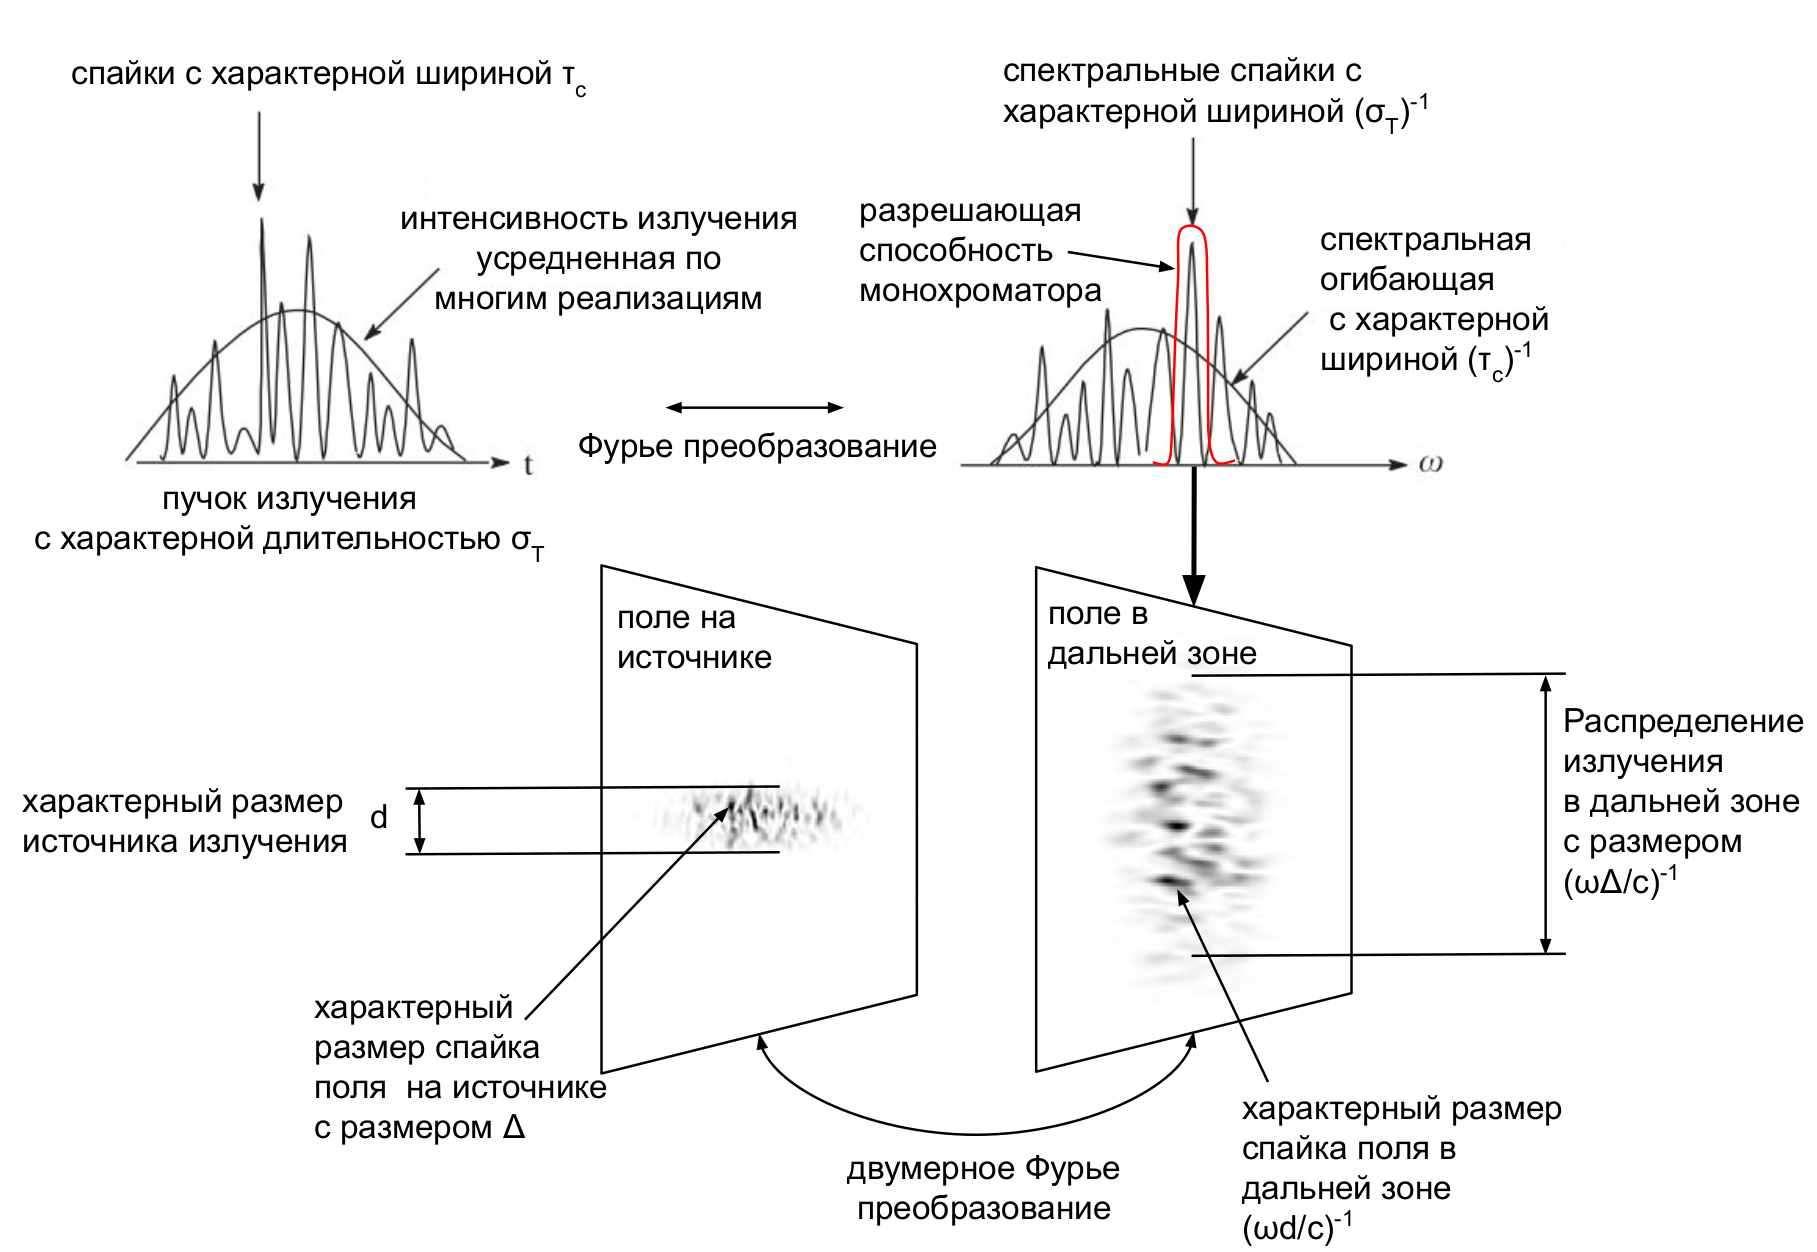
\includegraphics[width=0.99\linewidth]{spikes.png}
	\caption{Спайковая структура излучения синхротронного излучения. Красной линией показана полоса излучения, выделяемая монохроматором}
	\label{fig:spikes}
\end{figure}
\noindent В $t$-пространстве поле имеет внутреннюю структуру с характерным размером спайка, равным продольной длине когерентности излучения одного электрона, а характерная длительность поля, усреднённого по многим реализациям, определяется длительностью электронного сгустка. Ввиду связи $\omega t$-пространств, в $\omega$-пространстве размер спайка в спектре обратно пропорционален длительности излучения. Характерная огибающая спектра, после усреднения по многим реализациям, обратно пропорциональна длине когерентности излучения, такое соотношение -- следствие теоремы Винера-Хинчина. Если разрешить монохроматором спайк в $\omega$-пространстве, то на двумерном детекторе в дальней зоне можно увидеть поперечную спайковую структуру синхротронного излучения (Рис.~\ref{fig:spikes}). Это распределение с точностью до фазового фактора связано с распределением излучения на образце Фурье-преобразованием. В дальней зоне характерный размер спайка связан с размером источника излучения как:  $(\omega d /c)^{-1}$, и огибающая поля в дальней зоне связана с размером спайка на источнике как: $(\omega \Delta /c)^{-1}$, -- что является следствием обобщённой теоремы Ван Циттерта - Цернике. 


\newpage
%============================================================================================================================






